\documentclass[12pt, a4paper]{article}
\usepackage{pgf}
\usepackage{pgfpages}
\usepackage{tikz} % titlepage border
\usetikzlibrary{calc} % titlepage border
\usepackage{niceframe}
\usepackage{graphicx}
\usepackage{textcomp}
\usepackage{fancyhdr}
\usepackage{minitoc}
\usepackage{hyperref}
\usepackage{multicol}
\usepackage{sectsty}
\usepackage{adjustbox}%used for correct positioning of tables
\usepackage{titletoc}
\usepackage{adjustbox}%use to refined tables
\usepackage{float}
\usepackage{url}% solve missing $ in url
\usepackage{listings}% format source code, use with new custom command \code

%format source code inline
\newcommand{\code}[1]{\lstinline[language=C++, basicstyle=\color{orange!40!black}\ttfamily,morekeywords={cout,endl,\&,string},
keywordstyle=\color{blue},
commentstyle=\color{green!50!black},]{#1}}

% set default graphic path 
\graphicspath{ {./Pictures/} }


\sectionfont{\fontsize{20}{5}\selectfont}
\subsectionfont{\fontsize{15}{5}\selectfont}
\subsubsectionfont{\fontsize{12}{5}\selectfont}
\usepackage[a4paper, total={6in, 8in}]{geometry}
\newcommand\tab[1][0.5cm]{\hspace*{#1}}

%TitlePage

\begin{document}

\begin{titlepage}
    \begin{tikzpicture}[remember picture,overlay,inner sep=0,outer sep=0]
        \draw[blue!70!black,line width=4pt] ([xshift=-1.5cm,yshift=-2cm]current page.north east) coordinate (A)--([xshift=1.5cm,yshift=-2cm]current page.north west) coordinate(B)--([xshift=1.5cm,yshift=2cm]current page.south west) coordinate (C)--([xshift=-1.5cm,yshift=2cm]current page.south east) coordinate(D)--cycle;

        \draw ([yshift=0.5cm,xshift=-0.5cm]A)-- ([yshift=0.5cm,xshift=0.5cm]B)--
        ([yshift=-0.5cm,xshift=0.5cm]B) --([yshift=-0.5cm,xshift=-0.5cm]B)--([yshift=0.5cm,xshift=-0.5cm]C)--([yshift=0.5cm,xshift=0.5cm]C)--([yshift=-0.5cm,xshift=0.5cm]C)-- ([yshift=-0.5cm,xshift=-0.5cm]D)--([yshift=0.5cm,xshift=-0.5cm]D)--([yshift=0.5cm,xshift=0.5cm]D)--([yshift=-0.5cm,xshift=0.5cm]A)--([yshift=-0.5cm,xshift=-0.5cm]A)--([yshift=0.5cm,xshift=-0.5cm]A);


        \draw ([yshift=-0.3cm,xshift=0.3cm]A)-- ([yshift=-0.3cm,xshift=-0.3cm]B)--
        ([yshift=0.3cm,xshift=-0.3cm]B) --([yshift=0.3cm,xshift=0.3cm]B)--([yshift=-0.3cm,xshift=0.3cm]C)--([yshift=-0.3cm,xshift=-0.3cm]C)--([yshift=0.3cm,xshift=-0.3cm]C)-- ([yshift=0.3cm,xshift=0.3cm]D)--([yshift=-0.3cm,xshift=0.3cm]D)--([yshift=-0.3cm,xshift=-0.3cm]D)--([yshift=0.3cm,xshift=-0.3cm]A)--([yshift=0.3cm,xshift=0.3cm]A)--([yshift=-0.3cm,xshift=0.3cm]A);

    \end{tikzpicture}

    \centerline{\LARGE{\textbf{UNIVERSITY OF SCIENCE}}}
    \bigskip
    \centerline{\large{VIETNAM NATIONAL UNIVERSITY - HO CHI MINH CITY}}

    \centerline{\Large{--------------------------------------}}

    \bigskip

    \centerline{
\includegraphics[width=50mm]{logo.png}}

    \bigskip

    \centerline{\niceframe[11cm]
        {
            \begin{center}
                \LARGE{\textbf{BÁO CÁO NHÓM}}
                \linebreak
                \centering\LARGE{\textbf{ASSIGNMENT 5}}
            \end{center}
        }
    }

    \bigskip
    \bigskip

    \centerline{\LARGE{\textbf{HỆ THỐNG MÁY TÍNH}}}
    \raggedright
    \bigskip

    \begin{table}[h]
        \begin{adjustbox}{width=\columnwidth,center}
            \begin{tabular}{rrlc}
                 & Giảng viên      & Thái Hùng Văn       &          \\
                 &                 &                     &          \\
                 & Sinh viên       & Nguyễn Quốc Huy     & 21127511 \\
                 &                 & Lê Hoàng Sang       & 21127158 \\
            \end{tabular}
        \end{adjustbox}
    \end{table}
\end{titlepage}



%Header&Footer

\pagestyle{fancy}
\fancyhf{}
\addtolength{\topmargin}{-0.70894pt}
\setlength{\headheight}{12.70894pt}

\lhead{\textbf{FIT-HCMUS}}
\rhead{\textbf{ASSIGNMENT 5}}
\rfoot{\textbf{\thepage}}



%Tableofcontents

\tableofcontents

\pagebreak

\section{GIỚI THIỆU THÔNG TIN}

\subsection{Thành viên nhóm và thông tin liên lạc}
Gồm 2 thành viên thực hiện
\begin{itemize}
    \item 21127511 - Nguyễn Quốc Huy - nqhuy21@clc.fitus.edu.vn
    \item 21127158 - Lê Hoàng Sang - lhsang21@clc.fitus.edu.vn
\end{itemize}
\subsection{Nội dung bài tập}
\begin{figure}[H]
    \begin{center}
        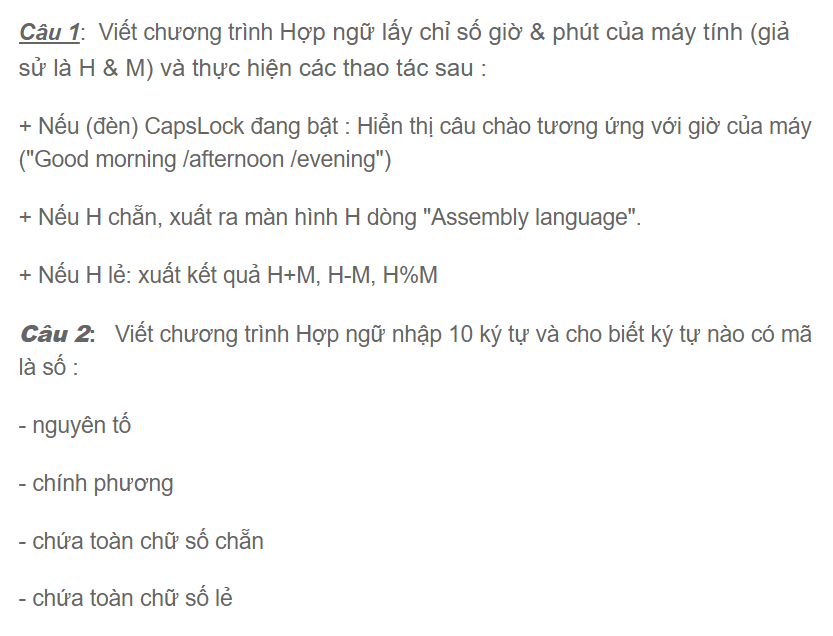
\includegraphics[scale = 1]{Topic.png}
    \end{center}
\end{figure}
\newpage
\subsection{Bảng phân công và mức độ hoàn thành}
\begin{table}[h]
    \begin{adjustbox}{width=\columnwidth,center}
        \begin{tabular}{lllcc}
            &\textbf{PHẦN}& \textbf{NỘI DUNG}                       &\textbf{THỰC HIỆN} & \textbf{HOÀN THÀNH} \\
            & Câu 1       & Kiểm tra đèn capslock                   &  Quốc Huy       & 100\%               \\
            &             & Xử lý thông tin khi giờ chẵn và lẻ      & Quốc Huy        & 100\%               \\
            &             &                                         &                 &                     \\ 
            & Câu 2       & Xử lý nhập, xuất 10 ký tự               & Hoàng Sang      & 100\%               \\
            &             & Kiểm tra ký tự có mã là số nguyên tố    & Hoàng Sang      & 100\%               \\
            &             & Kiểm tra ký tự có mã là số chính phương & Hoàng Sang      & 100\%               \\
            &             & Kiểm tra ký tự có mã toàn số chẵn       & Quốc Huy        & 100\%               \\
            &             & Kiểm tra ký tự có mã toàn số lẻ         & Quốc Huy        & 100\%               \\
        \end{tabular}
    \end{adjustbox}
\end{table}


\subsection{Các file chính chạy chương trình}

\begin{itemize}
    \item ex01.asm
    \item ex02.asm
\end{itemize}

\section{MÔ TẢ THUẬT TOÁN}
\subsection{CÂU 1}
\begin{itemize}
    \item Ý tưởng của bài này sẽ là sử dụng ngắt int 16h để lấy phím đè - ở đây là phím capslock
    \item Sử dụng ngắt int21h, ah = 2ch để lấy thời gian thực của hệ thống đồng thời gọi các hàm chức năng để tính toán và in ra màn hình theo yêu cầu đề bài.
    \item Sử dụng nhiều nhãn dán(label) để đảm bảo độ chính xác của chương trình.
    \item Sử dụng nhiều hàm để cho chương trình được gọn hơn, bao gồm: 
    \begin{itemize}
        \item Hàm main: Là hàm chính chứa đủ các bước theo yêu cầu đề bài.
        \item Hàm Hour: Chuẩn bị gán các thanh ghi để xử lý thông tin cho việc in giờ.
        \item Hàm Hien\_Thi\_So\_Gio: In ra màn hình số giờ, hàm này thực hiện kể cả trong trường hợp giờ có 2 chữ số.
        \item Hàm Minute: Chuẩn bị gán các thanh ghi để xử lý thông tin cho việc in phút.
        \item Hàm Hien\_Thi\_So\_Gio: In ra màn hình số phút, hàm này thực hiện kể cả trong trường hợp phút có 2 chữ số.
        \item Hàm Loi\_Chao: Hàm hiển thị các lời chào theo giờ tương ứng.
        \item Hàm Gio\_Chan: Hàm nếu là giờ chẵn thì xử lý thông tin theo yêu cầu đề bài.
        \item Hàm Gio\_Le: Hàm nếu là giờ lẻ thì xử lý thông tin theo yêu cầu đề bài.
    \end{itemize}
    \item Sử dụng thêm phép toán đặc biệt: pop và push để tiện cho việc in số có 2 ký tự trở lên:
    \begin{itemize}
        \item Đầu tiên sẽ lấy ký tự cần in chia 10, phần dư sẽ được push vào ngăn xếp.
        \item Sau đó tăng biến đếm và lặp lại vòng lặp push từng ký tự vào cho đến khi không còn ký tự nào.
        \item Tiếp theo dựa vào số biến đếm đã đếm được, lần lượt pop ra và in từng ký tự
        \item Mỗi lần in ký tự cần cộng thêm 30h để chuyển thành số.
    \end{itemize}
    \item Các trường hợp về giờ chẵn, giờ lẻ đã được kiểm tra qua và hoàn thành.
    \begin{figure}[H]
        \begin{center}
            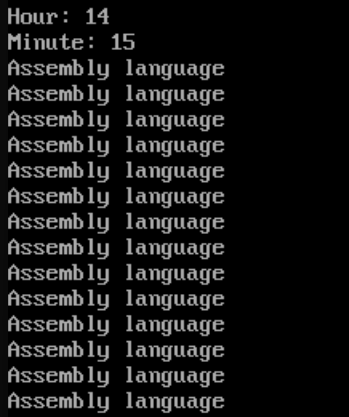
\includegraphics[scale = 2]{GioChan.png}
        \end{center}
    \end{figure}
    \begin{figure}[H]
        \begin{center}
            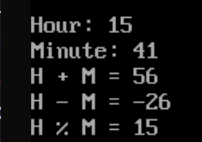
\includegraphics[scale = 2]{GioLe.png}
        \end{center}
    \end{figure}
\end{itemize}
\begin{itemize}
    \item Các bước chi tiết đã được ghi chú(comment) trong code.
\end{itemize}
\subsection{CÂU 2}
\begin{itemize}
    \item Thao tác chính của bài này là vấn đề về nhập xuất và xử lý 10 ký tự, vậy nên phương pháp tối ưu nhất là sử dụng mảng.
    \item Ý tưởng của bài này là nhập 10 số vào mảng, sau đó sẽ gọi các hàm để kiểm tra
    \item Sử dụng nhiều nhãn dán(label) để đảm bảo độ chính xác của chương trình.
    \item Sử dụng nhiều hàm để cho chương trình được gọn hơn, bao gồm: 
    \begin{itemize}
        \item Hàm main: hàm chính, chứa các lời gọi hàm, nhập xuất, vòng lặp, kết thúc chương trình... 
        \item Hàm CheckSNT: kiểm tra xem có phải là Số nguyên tố hay không.
        \item Hàm CheckSquare: kiểm tra xem có phải là Số chính phương hay không. 
        \item Hàm CheckEven: kiểm tra xem các kí tự trong mảng có phải bao gồm tất cả Số chẵn không. 
        \item Hàm CheckOdd: kiểm tra xem các kí tự trong mảng có phải bao gồm tất cả Số lẻ không. 
    \end{itemize}
    \item Sau mỗi hàm thì sẽ duyệt lại các phần tử trong mảng để đảm bảo không bỏ sót phần tử nào.
    \item Dưới đây là minh họa khi nhập 1 chuỗi 10 ký tự:
    \begin{figure}[H]
        \begin{center}
            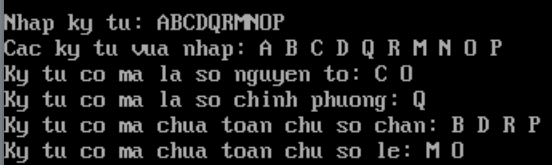
\includegraphics[scale = 1.5]{Kytu.png}
        \end{center}
    \end{figure}
    \normalsize{
    Như ta thấy, ký tự A và N có mã Ascii là 65 và 78 nên không thuộc bất cứ trường hợp nào.\\
    Ký tự C và O có mã là 67 và 79 nên thuộc trường hợp số nguyên tố.\\
    Ký tự Q có mã là 81 nên nó là số chính phương.\\
    Ký tự B(66), D(68), P(80) và R(82) đều có mã toàn các số chẵn.\\
    Ký tự M(77) và O(79) đều có mã toàn các số lẻ.\\
    }
    \item Ví dụ khác:
    \begin{figure}[H]
        \begin{center}
            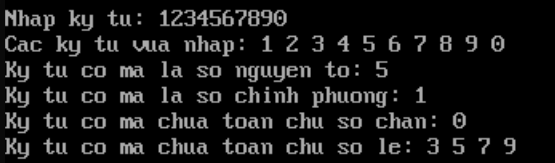
\includegraphics[scale = 1.5]{Vidu.png}
        \end{center}
    \end{figure}
\end{itemize}
\begin{itemize}
    \item Các bước chi tiết đã được ghi chú(comment) trong code.
\end{itemize}

\section{THAM KHẢO}
\textbf{Các thao tác cơ bản}: \url{https://www.jundat95.com/2015/10/mot-so-lenh-co-ban-trong-lap-trinh.html }\\
\textbf{Sử dụng mảng}: \\\url{https://cachhoc.net/2013/09/12/assembly-xuat-mang-trong-assembly/}\\ \url{https://www.tutorialspoint.com/assembly_programming/assembly_arrays.htm }\\
\textbf{Tìm hiểu các ngắt và phép toán hợp ngữ}: \\\url{https://yassinebridi.github.io/asm-docs/}\\
\textbf{In ký tự có mã 2 ký tự}:\\\url{https://cachhoc.net/2013/09/12/assembly-xuat-so-co-nhieu-chu-so-trong-assembly/}\\
\bigskip
\bigskip
\bigskip

\begin{center}
    \LARGE{Hết! Xin cảm ơn}
\end{center}
\end{document}